% (les classes i operacions) (pot ser minimalista, es normal que sigui prima)(simplement tinc els controladors)(es poc mantenible i extensible, pero rapid de desenvolupar)
% \begin{titlebox}{TODO}
%   Explain classes, components, how the code is structured, and where each thing is and runs.
% \end{titlebox}

% % Tb explicar lo de heroku aquí
% % No dir que ho tinc tot en un arxiu
% % inventarme les classes 

% \begin{titlebox}{TODO}
%   Do a sequence diagram of an example user story. To showcase how everything works. (Create subject)
% \end{titlebox}

% \begin{titlebox}{TODO}
%   Do a sequence diagram of the classes and where they are
% \end{titlebox}

In this project, the domain layer is very thin because the app doesn't have many entities.

The main entity is the subject class. It contains the information about the subject, the user's grades, and functions to make calculations with the grades, like calculating the final grade.

The diagram in figure \ref{fig:class-diagram} is a summarized version of the domain layer, it doesn't contain all the actual methods.

\vfill
\begin{figure}[H]
    \center
    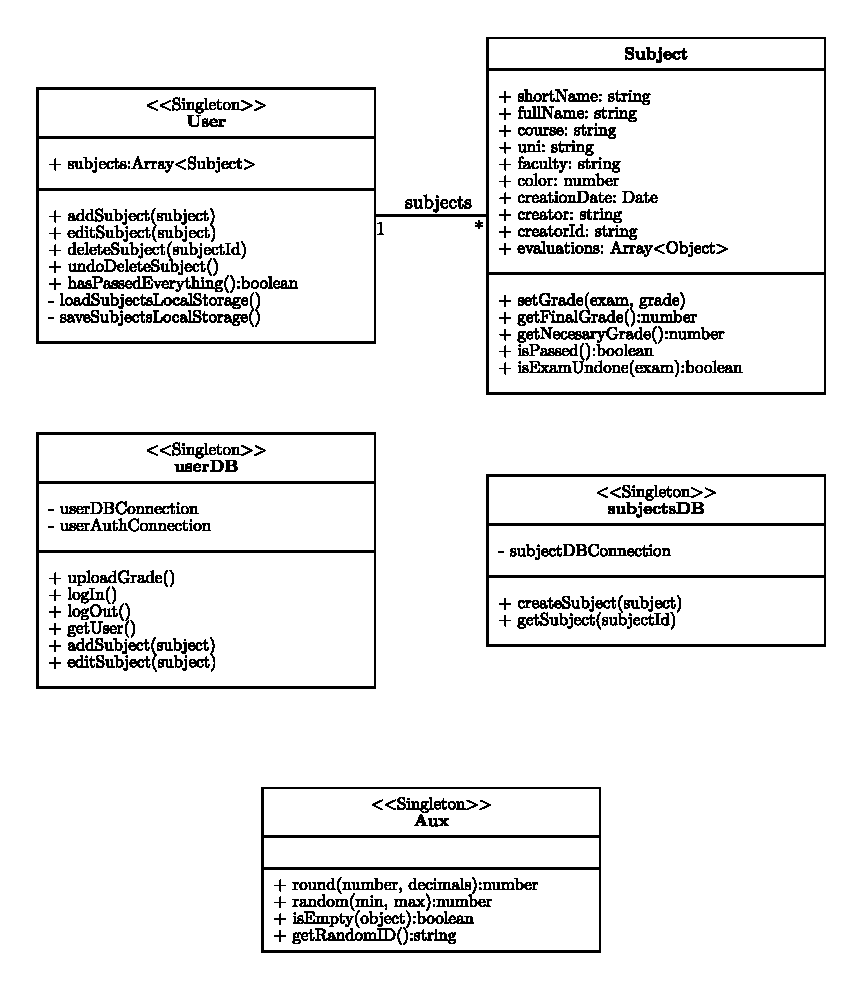
\includegraphics[height=15cm]{media/diagrams/class-diagram.pdf}
    \caption{Classes diagram}
    \label{fig:class-diagram}
\end{figure}
\vfill
